\begin{figure}[!h]
    \centering
    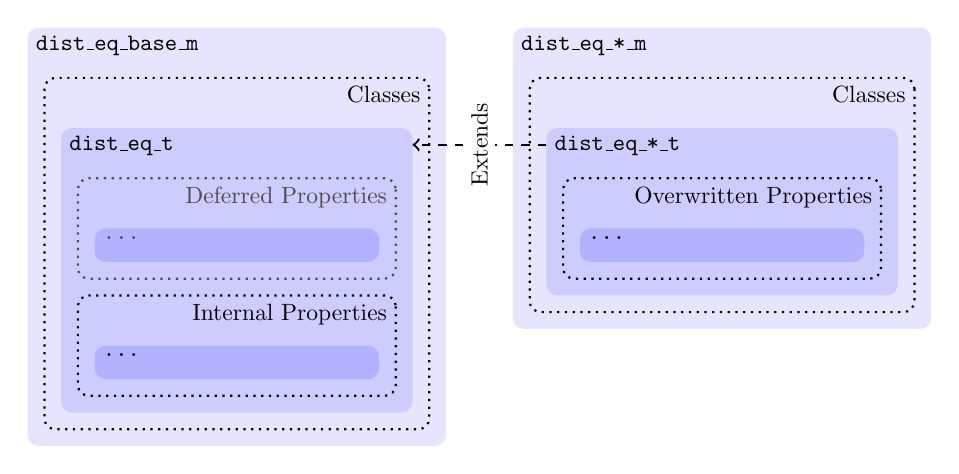
\begin{tikzpicture}[scale = 0.85, every node/.style = {scale = 0.85}, every text node part/.style = {align = left}]
        \fill[rounded corners, fill = blue!10]
            (0, 0) node[below right] {\tt dist\_eq\_base\_m}
            rectangle
            (6.25, -6.25);
            \draw[rounded corners, dotted, thick]
                (6, -0.75) node[below left] {Classes}
                rectangle
                (0.25, -6);
                \fill[rounded corners, fill = blue!20]
                    (0.5, -1.5) node[below right] {\tt dist\_eq\_t}
                    rectangle
                    (5.75, -5.75);
                    \draw[rounded corners, dotted, thick, dotted, black!70]
                        (5.5, -2.25) node[below left] {Deferred Properties}
                        rectangle
                        (0.75, -3.75);
                        \fill[rounded corners, fill = blue!30]
                            (1, -3) node[below right] {}
                            rectangle
                            (5.25, -3.5);
                        \node[black!70] at (1, -3) [below right] {
                                {\tt ...}
                            };
                    \draw[rounded corners, dotted, thick]
                        (5.5, -4) node[below left] {Internal Properties}
                        rectangle
                        (0.75, -5.5);
                        \fill[rounded corners, fill = blue!30]
                            (1, -4.75) node[below right] {}
                            rectangle
                            (5.25, -5.25);
                        \node at (1, -4.75) [below right] {
                                {\tt ...}
                            };
        \fill[rounded corners, fill = blue!10]
            (7.25, 0) node[below right] {\tt dist\_eq\_*\_m}
            rectangle
            (13.5, -4.5);
            \draw[rounded corners, dotted, thick]
                (13.25, -0.75) node[below left] {Classes}
                rectangle
                (7.5, -4.25);
                \fill[rounded corners, fill = blue!20]
                    (7.75, -1.5) node[below right] {\tt dist\_eq\_*\_t}
                    rectangle
                    (13, -4);
                    \draw[rounded corners, dotted, thick]
                        (12.75, -2.25) node[below left] {Overwritten Properties}
                        rectangle
                        (8, -3.75);
                        \fill[rounded corners, fill = blue!30]
                            (8.25, -3) node[below right] {}
                            rectangle
                            (12.5, -3.5);
                        \node at (8.25, -3) [below right] {
                                {\tt ...}
                            };
        \draw[->, thick, dashed]
            (7.75, -1.75) -- (5.75, -1.75)
            node[midway, rotate = 90, fill = white] {Extends};
    \end{tikzpicture}
\end{figure}